% !Mode:: "TeX:UTF-8"
%% 请使用 XeLaTeX 编译本文.
\documentclass{WHUMaster}   % 选项 forprint: 交付打印时, 建议加上此选项, 以消除彩色链接文字, 避免彩色字迹打印偏淡.
                                              % 选项 forlib: 提交给图书馆的电子版, 需要加上选项 forlib, 以消除空白页和彩色链接.
                                              % 选项 smd: Specialist Master's Degree, 产生专业硕士学位论文封面、页眉.
%%%=== 参考文献=== %%%
\bibliographystyle{abbrv}        % 参考文献样式,  plain,unsrt,alpha,abbrv 等等
%%%%%%%%%%%%%%%%%%%%%%%%%%%%%%%%%%%%%%%%%%%%%%%%%%%%
\begin{document}
%%%%%%%-------------------------------------------------

\fenleihao{O159}  % 分类号:《中国图书资料分类法》的类号. 必填. 要根据自己的学科方向填写!!
\miji{}                % 密级
\UDC{}               %《国际十进制分类法UDC》的类号. 选填.
\bianhao{10486}  % 学校编号, 10486是武汉大学的编号. 不用改动.

\title{武汉大学硕士论文~\LaTeX~模板}
\Etitle{A \LaTeX~Thesis Template for Wuhan University} % 英文题目
\author{刘佳迎}
\StudentNumber{0121710880223}   % 学号
\Eauthor{HUANG Zhenghua}            %作者英文名
\Csupervisor{胡宝清\quad 教授}        %指导教师中文名、职称
\Esupervisor{Prof.~HU Bao Qing}     %指导教师英文名、职称
\Cmajor{计算数学}                          % 专业中文名[ SMD:专业类别(领域)]
\Emajor{Computational Mathematics}% 专业英文名[ SMD:专业类别(领域)]
\Cspeciality{智能计算}                     % 研究方向
\Especiality{Intelligent Computing}   % 研究方向
\Schoolname{School of Mathematics and Statistics} %学院英文名. 不确定的话, 请看一下自己学院的网页上是怎么写的. 别搞错了!
\date{二〇一六年五月}                    % 硕士类只写年月. 要注意和英文日期一致!!
\Edate{May, 2016}                   % 英文封面日期

%-----------------------------------------------------------------------------
\pdfbookmark[0]{封面}{title}         % 封面页加到 pdf 书签
\maketitle
%-----------------------------------------------------------------------------
% !Mode:: "TeX:UTF-8"

%%% 此部分包含: (1) 英文封面 (无需改动) ; (2) 郑重声明 (无需改动).

%%%%%%%%%%%%%%%%%%%%%%%%%%%%%
%%% -------------  英文封面 (无需改动)-------------   %%%
%%%%%%%%%%%%%%%%%%%%%%%%%%%%%
\thispagestyle{empty}
\renewcommand{\baselinestretch}{1.5}  %下文的行距
\vspace*{0.5cm}

\begin{center}{\zihao{2} \the\Etitle \par}\end{center}

\vfill

\begin{center}
\zihao{4}
\begin{tabular}{ r l }
 Candidate:      &  {\sc \the\Eauthor}      \\
 Student Number: & {\the\StudentNumber} \\
 Supervisor:     &  {\sc \the\Esupervisor}   \\
 Major:          & \the\Emajor  \\
\ifsmd \else Speciality:     & \the\Especiality \fi
\end{tabular}

\vspace*{2cm}
\begin{center}
  \iflib % 向图书馆提交电子文档, 使用黑白校徽.
  
\includegraphics[height=4cm]{whu.eps}       %%  黑白的. 很小, 只有 10k.
  \else
     \ifprint % 文档打印, 使用黑白校徽.
  
\includegraphics[height=4cm]{whu.eps}       %%  黑白的.
  \else
  
\includegraphics[height=4cm]{whulogo.eps} %%  彩色的.
  \fi
  \fi
\end{center}


\zihao{-2}
\the\Schoolname\\
{\sc Wuhan University}

\vspace*{1.0cm}

\the\Edate

\end{center}
%%%%%%%--判断是否需要空白页-----------------------------
  \iflib
  \else
  \newpage
  \thispagestyle{empty}
  \cleardoublepage
  \fi
%%%%%%%-------------------------------------------------
%%%--- 加入``郑重声明'' --- %%%%%%%%%%%%%%%%%
{\pagestyle{empty}
\newpage
\vspace*{20pt}
\begin{center}{\ziju{0.8}\zihao{-2}\heiti 论文原创性声明}\end{center}
\par\vspace*{30pt}
\renewcommand{\baselinestretch}{2}
{\zihao{4} \songti %


本人郑重声明: 所呈交的学位论文, 是本人在导师指导下, 独立进行研究工作所取得的研究成果.
除文中已经标明引用的内容外, 本论文不包含任何其他个人或集体已经发表或撰写过的研究成果.
对本文的研究做出贡献的个人和集体, 均已在文中以明确方式标明. 本声明的法律结果由本人承担.


\vskip2cm

\hspace*{4cm}学位论文作者(签名): \hspace{4cm} \hfill \\[1cm]
\hspace*{10cm}年 \hfill  月 \hfill 日\hspace{1cm}\hfill\par}

%%%%%%%--判断是否需要空白页-----------------------------
  \iflib
  \else
  \newpage
  \cleardoublepage
  \fi
%%%%%%%-------------------------------------------------
}
\renewcommand{\baselinestretch}{1.6}
\small\normalsize




    % 加入英文封面
\frontmatter
\pagenumbering{Roman}               % 正文之前的页码用大写罗马字母编号.

\cleardoublepage
\newpage  \pagestyle{fancy} \fancyfancy
%------------------------------------------------------------------------------
% !Mode:: "TeX:UTF-8"

%%% 说明: 此部分需要自己填写的内容:  (1) 中文摘要及关键词 (2) 英文摘要及关键词

%%%%%%%%%%%%%%%%%%%%%%%
%%% ------------ 中文摘要 ---------------%%%
%%%%%%%%%%%%%%%%%%%%%%%
\begin{cnabstract}
本文主要介绍和讨论了武汉大学硕士毕业论文的~\LaTeX~模板.
指明了编译方法, 强调了公式排版的一些细节问题, 也指出了一些常见的排版错误.



\end{cnabstract}
\vspace{1em}\par\vfill

%%%--------- 关键词 -------- %%%
\cnkeywords{毕业论文, \LaTeX{}, 模板, XeLaTeX }

%%%%%%%%%%%%%%%%%%%%%%%


%%%%%%%%%%%%%%%%%%%%%%%
%%% ------------ 英文摘要 ---------------%%%
%%%%%%%%%%%%%%%%%%%%%%%

\begin{enabstract}
This thesis is a study on the theory of \dots.




\end{enabstract}
\vspace{1em}\par\vfill

%%%------ 英文关键词 ------- %%%
\enkeywords{\LaTeX{}, XeLaTeX, \dots}


      % 加入中英文摘要.
%---把目录加入到书签---%%%%%%%%%%%%%%
\pdfbookmark[0]{目录}{toc}%%%%%%%%%%%%

\tableofcontents

%------------------------------------------------------------------------------
\mainmatter %% 以下是正文
\baselineskip=20pt  % 正文行距为 20 磅
%%%%%%%%%%%%%%%%%%%%%%%%%%%%%%%%%%%%
\chapter{先说重要的}

\section{具体使用步骤}
\begin{description}

  \item[Step 1]  进入 includefile 文件夹,  打开 midmatter.tex,  backmatter.tex 这两个文档,
        分别填写 (1) 中文摘要、英文摘要, (2) 致谢.

  \item[Step 2]  打开主文档 MasterTemplate.tex, 填写题目、作者等等信息, 书写正文.

  \item[Step 3]  使用 XeLaTeX 编译. 具体见 \ref{sec-compile} 节.


\end{description}




\section{编译的方法}\label{sec-compile}

默认使用 XeLaTeX 编译, 直接生成~pdf 文件.

若另存为新文档, 请确保文档保存类型为 \verb|:UTF-8|. 当然目前很多编辑器默认文字编码为 UTF-8.
WinEdt 9.0 之后的版本都是默认保存为 UTF-8 的.



\section{文档类型选择}
文档类型有 3 种情形:

\begin{table}[ht]\centering
\begin{tabular}{ll}
\hline
   \verb|\documentclass{WHUMaster}|                 &  硕士论文 \\
   \verb|\documentclass[forprint]{WHUMaster}|    &  硕士论文打印版  \\
   \verb|\documentclass[forlib]{WHUMaster}|       &  硕士论文图书馆提交版  \\
\hline
\end{tabular}
\end{table}

另外: 专业硕士毕业论文, 请在上述情形另外加上选项 smd. 专业硕士毕业论文的封面稍有不同(中英文封面), 页眉也顺势改变了. 即
\begin{table}[ht]\centering
\begin{tabular}{ll}
\hline
   \verb|\documentclass[smd]{WHUMaster}|               &  专业硕士论文 \\
   \verb|\documentclass[smd,forprint]{WHUMaster}|    &  专业硕士论文打印版  \\
   \verb|\documentclass[smd,forlib]{WHUMaster}|       &  专业硕士论文图书馆提交版  \\
\hline
\end{tabular}
\end{table}



相关解释见接下来的两节.



\section{打印的问题}
\begin{enumerate}[i)]
  \item  硕士论文要求\colorbox{yellow}{双面打印}.
  \item  关于文档选项 forprint: 交付打印时, 建议加上选项 forprint, 以消除彩色链接文字, 避免打印字迹偏淡.
  \item  打印时留意不要缩小页面或居中. 即页面放缩方式应该是``无''(Adobe Reader XI 是选择``实际大小'').
           有可能页面放缩方式默认为``适合可打印区域'', 会导致打印为原页面大小的 $97\%$.
           文字不要居中打印, 是因为考虑到装订, 左侧的空白留得稍多一点(模板已作预留).
\end{enumerate}

\textbf{问}: {\kaishu 生成 PDF 文件时,不能去掉目录和文章的引用彩色方框,请问怎么解决?}

\textbf{答}: {\kaishu 方框表示超级链接, 只在电脑上看得见. 实际打印时, 是没有的.}





\section{提交电子文档}

向武汉大学图书馆提交电子文档, 需单独编译文件: 在文档选项中添加 forlib.

原因: 图书馆要求提交的电子文档不能有空白页、彩色文字.

({\kaishu 这个要求使我在编制模板时遇到了一点问题: 这会导致电子版与纸质版的页码不一致.  论文每章的起始页默认在奇数页, 这会不可避免地出现空白页.})


本文档下载更新地址: \url{http://aff.whu.edu.cn/huangzh/}. 使用之前, 请移步查看是否有更新.

问题反馈及建议, 请联系: huangzh@whu.edu.cn.




\chapter{杂七杂八的话}

\section{Readme}

模板文件的结构, 如下表所示:
 \begin{table}[ht]\centering
\begin{tabular}{r|r|l}
\hline\hline
  \multicolumn{2}{l|}{MasterTemplate.tex }  &  主文档. 在其中填写正文.\\\hline
                          &frontmatter.tex&  英文封面. \hfill ({\kaishu 无需干预}) \\\cline{2-3}
 includefile 文件夹  & midmatter.tex  &  中文摘要, 英文摘要.\hfill  ({\kaishu 自行填写}) \\\cline{2-3}
                            & backmatter.tex &  致谢.\hfill  ({\kaishu 自行填写}) \\\hline
  \multicolumn{2}{l|}{figures 文件夹} &  存放图片文件.\\\hline
  \multicolumn{2}{l|}{BIBbase 文件夹} &   供 BibTeX{} 做参考文献时选用.\\
\hline
  \multicolumn{2}{l|}{WHUMaster.cls} &  定义文档格式的 class file. 不可删除.\\ \hline \hline
\end{tabular}
\end{table}
%  \footnotetext[1]{定制这个参考文献格式, 主要是希望尽可能满足武汉大学硕士论文的相应格式要求, 比如要求将~article 的``年份''写在``卷号''之前.
%                   存在的问题是: 无法将~book 的``出版时间''标在``出版单位''之前. 事实上, 这个要求有悖于``国家标准~7714-87 文后参考文献著录规则''.
%                   作者名的写法, 依照了``文后参考文献著录规则'', 比如~Albert Einstein 写为~Einstein A.}
%  \footnotetext[1]{编译信息文件常常让我们的文件夹变得凌乱不堪, WinEdt窗口的``垃圾箱''按钮(Erase Output Files),
%     可以让我们方便地删除这些``垃圾''文件. 这也减少了误删文件的可能.}

无需也不要改变、移动上述文档的位置.



可能这里的文档看上去有点多. 如果不习惯用~\verb|\include{ }|~的方式加入``子文档'', 当然可以把它们合并在主文档, 成为一个文档.
({\kaishu 但是这样并不会给我们带来方便.})

利用~WinEdt~的~Project tree, 可以方便地管理这些文件:
\begin{itemize}
    \item 点击~WinEdt~窗口的~Project Tree~按键;
    \item 再点击~WinEdt~窗口的~Set Main File~按键;
\end{itemize}
接下来的管理, 已经清楚地展示在跳出的窗口中了. 再去处理其他的文件时, 还要点击~WinEdt~窗口的~Remove Main File~按键.


英文封面页加了校徽, 有黑白、彩色两种备选, 都是矢量图形, 放大不会失真. 图片文件很小,
用~MetaPost~生成的(准确的说, 是最后一道工序用到了~MetaPost), 过程有点复杂.
封面上毛体字的``武汉大学''也是这样做出的. 



2016 年 02 月更新: 调整为适应 TeX Live 2015 的版本.

2016 年 04 月更新: 按照研究生院新发布的要求进行改造. 主要变化: (1) 封面``武汉大学''字样改为毛体题字;
(2) 郑重声明改为论文原创性声明; (3) 加了页眉; (4) 专业硕士论文封面, 供选择. 使用选项 smd 即可.

\section{字体调节}

\begin{tabular}{ll}
 \verb|\songti| & {\songti 宋体} \\
 \verb|\heiti| & {\heiti 黑体} \\
 \verb|\fangsong| & {\fangsong 仿宋} \\
 \verb|\kaishu| & {\kaishu 楷书} \\
\end{tabular}


\section{字号调节}
字号命令: \verb|\zihao|

\begin{tabular}{ll}
\verb|\zihao{0}| &\zihao{0}  初号字 English \\
\verb|\zihao{-0}|&\zihao{-0} 小初号 English \\
\verb|\zihao{1} |&\zihao{1}  一号字 English \\
\verb|\zihao{-1}|&\zihao{-1} 小一号 English \\
\verb|\zihao{2} |&\zihao{2}  二号字 English \\
\verb|\zihao{-2}|&\zihao{-2} 小二号 English \\
\verb|\zihao{3} |&\zihao{3}  三号字 English \\
\verb|\zihao{-3}|&\zihao{-3} 小三号 English  \\
\verb|\zihao{4} |&\zihao{4}  四号字 English  \\
\verb|\zihao{-4}|&\zihao{-4} 小四号 English \\
\verb|\zihao{5} |&\zihao{5}  五号字 English \\
\verb|\zihao{-5}|&\zihao{-5} 小五号 English \\
\verb|\zihao{6} |&\zihao{6}  六号字 English \\
\verb|\zihao{-6}|&\zihao{-6} 小六号 English \\
\verb|\zihao{7} |&\zihao{7}  七号字 English \\
\verb|\zihao{8} |&\zihao{8}  八号字 English \\
\end{tabular}



\section{已加入的常用宏包}

\begin{description}
%  \item[amsmath,amssymb]
  \item[cite]  参考文献引用, 得到形如 [3-7] 的样式.
  \item[color,xcolor]  支持彩色.
  \item[enumerate]  方便自由选择 enumerate 环境的编号方式. 比如

  \verb|\begin{enumerate}[(a)]| 得到形如 (a), (b), (c) 的编号.

  \verb|\begin{enumerate}[i)]| 得到形如 i), ii), iii) 的编号.

\end{description}

另外要说明的是,  itemize, enumerate, description 这三种 list 环境, 已经调节了其间距和缩进,
以符合中文书写的习惯.

\section{标点符号的问题}

建议使用半角的标点符号, 后边再键入一个空格. 特别是在英文书写中要注意此问题!

使用半角也有不足的地方, 比如顿号出不来, 需要临时切换到全角. (当然也有输入法不需要切换, 比如紫光拼音, 可以直接用拼音输入逗号.)

双引号是由两个左单引号、两个右单引号构成的: \verb|``  ''|. 左单引号在键盘上数字~1 的左边.

但是, 无论您偏向于全角或半角, 强烈建议您使用实心的句号, 只要您书写的是自然科学的文章.
原因可能是因为, 比如使用全角句号的句子结尾处的``$x$。''容易误为数学式~$x_0$(\verb|$x_0$|)吧.

\section{中英文间距问题}

自动加入间距. 不再需要在公式、英文前后加字符``\verb|~|''或空格.

\section{引用的问题}


\subsection{参考文献的引用}

参考文献的引用, 用命令~\verb|\cite{ }|. 大括号内要填入的字串, 是自命名的文献条目名.

比如, 通常我们会说:

 {\kaishu
关于此问题, 请参见文献 \cite{r2}. 作者某某还提到了某某概念\upcite{r1}.}


上文使用的源文件为:

 {\kaishu
关于此问题, 请参见文献~\verb|\cite{r2}|. 作者某某还提到了某某概念~\verb|\upcite{r1}|.
}

其中~\verb|\upcite| 是自定义命令, 使文献引用呈现为\CJKunderdot{上标形式}.

({\heiti 注意:} {\kaishu 这里文献的引用, 有时需要以上标形式出现, 有时需要作为正文文字出现, 为什么?})

另外, 要得到形如~\cite{r1,r3,r4,r5} 的参考文献连续引用, 需要用到 cite 宏包(模板已经加入),
在正文中使用~\verb|\cite{r1,r3,r4,r5}| 的引用形式即可.
或者, 连续引用的上标形式: 使用~\verb|\upcite{r1,r2,r3}|, 得到\upcite{r1,r2,r3}.

\subsection{定理和公式的引用}

\begin{theorem}[谁发现的]\label{th-abcd}
最大的正整数是~$1$.
\end{theorem}

\begin{proof}
要找到这个最大的正整数, 我们设最大的正整数为~$x$, 则~$x \geqslant 1$, 两边同时乘以~$x$, 得到
\begin{equation}\label{eq-abc}
x^2 \geqslant x.
\end{equation}
而~$x$ 是最大的正整数, 由~\eqref{eq-abc} 式得到
\[
x^2 = x.
\]
所以
\begin{equation*}
x = 1.
\end{equation*}
\end{proof}

定理~\ref{th-abcd} 是一个重大的发现.

%%%%----- 定义等环境的举例 --------
\begin{definition}[整数]
 正整数(例如 1, 2, 3)、负整数(例如 ${−1}$, $−2$, $−3$)与零(0)合起来统称为{\heiti 整数}.
\end{definition}

\begin{remark}
  整数集合在数学上通常表示为 $\mathbf{Z}$ 或 $\mathbb{Z}$, 该记号源于德语单词 Zahlen(意为``数'')的首字母.
\end{remark}

\begin{proposition}
任意两个整数相加、相减、相乘的结果, 仍然是整数.
\end{proposition}

\begin{example}
  $1+2=3$.
\end{example}

\begin{corollary}
   在整数集合内, 相加、相减、相乘运算是封闭的.
\end{corollary}

\section{图形与表格}

支持 eps, pdf, jpg 这几种常见图形格式.

再次澄清一个误会: \LaTeX{} 支持的图形格式绝非 eps 这一种. 无需特意把图片转化为 eps 格式.

用形如 \verb|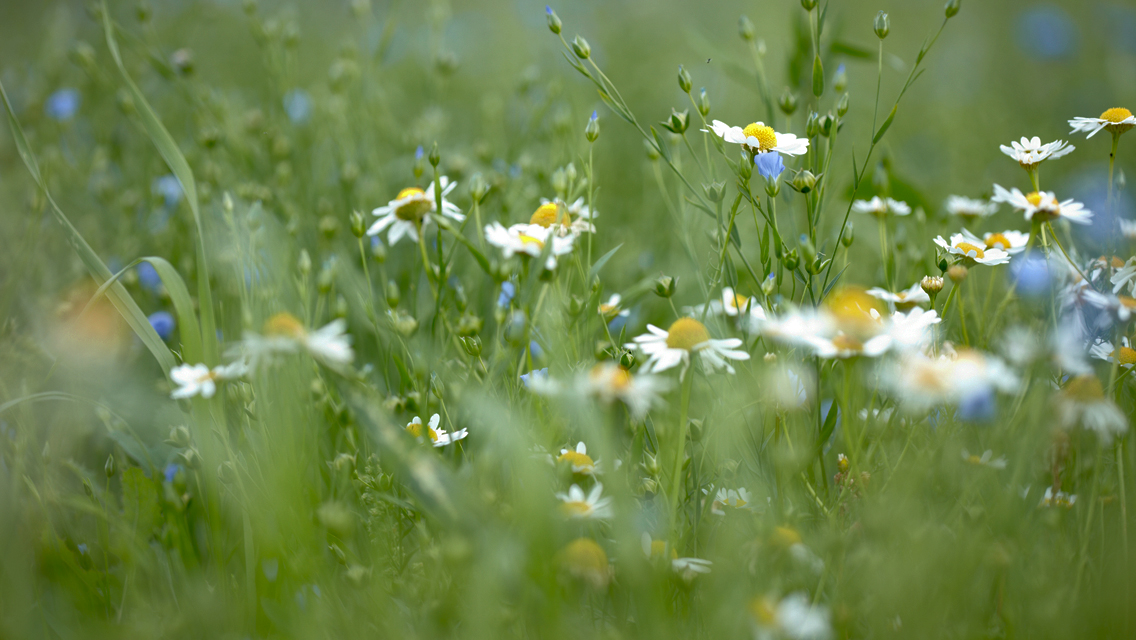
\includegraphics[width=12cm]{Daisy.jpg}| 的命令可以纳入图片.

如图 \ref{fig:1} 是一个纳入~jpg 图片的例子.

\begin{figure}[ht]
\centering
  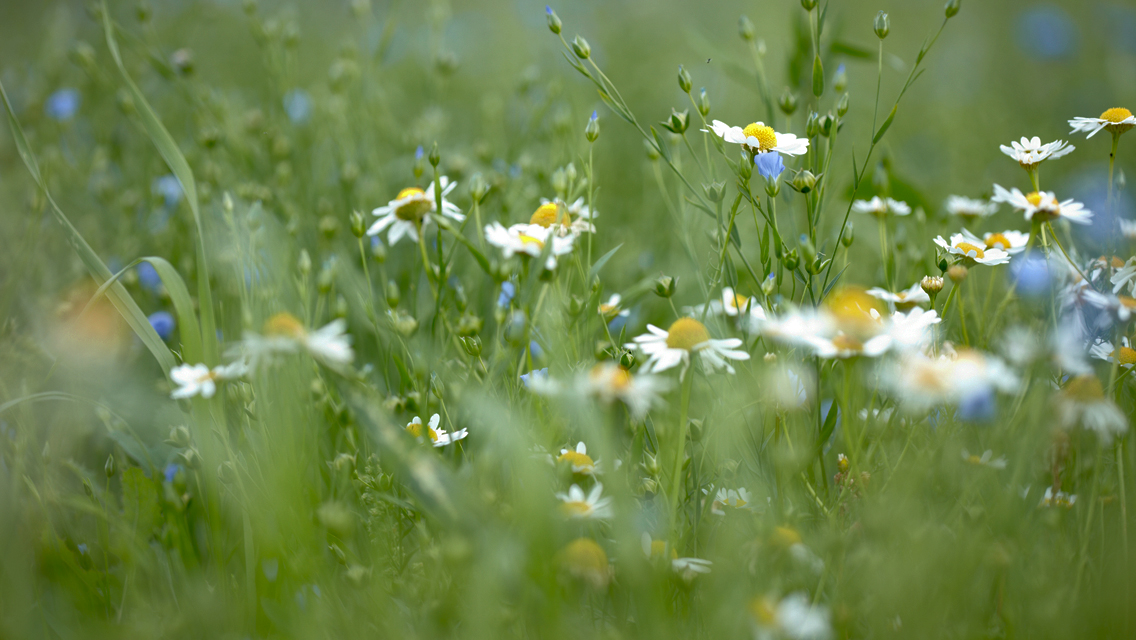
\includegraphics[width=\textwidth]{Daisy.jpg}
  \caption{一个彩色 jpg 图片的例子}
  \label{fig:1}
\end{figure}

表格问题, 建议使用``三线表'', 如表 \ref{tab:1}.

\begin{table}[ht]
\centering
\caption{一般三线表}
\label{tab:1}
    \begin{tabular}{c c c c c c c c c c c}
    \hline
    123 & 4  & 5  & 123 & 4 & 5123 & 4 & 5 & 123 & 4 & 5\\
    \hline
    67 & 890 & 13 & 123 & 4 & 5123 & 4 & 5 & 123 & 4 & 5\\
    67 & 890 & 13 & 123 & 4 & 5123 & 4 & 5 & 123 & 4 & 5\\
    67 & 890 & 13 & 123 & 4 & 5123 & 4 & 5 & 123 & 4 & 5\\
    \hline
    \end{tabular}
\end{table}

%\begin{table}[h]
%  \centering
%  \caption{调整线宽的三线表}\label{tab:2}
%    \begin{tabular}{c c c c c c c c c c c}
%    \hlinewd{0pt}
%    姓名: &&&&年龄: &&&& 性别:\\
%    \hlinewd{1.5pt}
%    123 & 4  & 5  & 123 & 4 & 5123 & 4 & 5 & 123 & 4 & 5\\
%    \hlinewd{1pt}
%    67 & 890 & 13 & 123 & 4 & 5123 & 4 & 5 & 123 & 4 & 5\\
%    67 & 890 & 13 & 123 & 4 & 5123 & 4 & 5 & 123 & 4 & 5\\
%    67 & 890 & 13 & 123 & 4 & 5123 & 4 & 5 & 123 & 4 & 5\\
%    \hlinewd{1.5pt}
%    \end{tabular}
%\end{table}

%\section{论文电子版提交的格式问题}
%
%《武汉大学博、硕士研究生学位论文缴送办法》要求``电子版应采用~Word97 或~Word2000 格式(DOC)编辑''\footnote{那已经是~2005 年的事情了.}.
%关于这个重要的问题, 我已致信武汉大学图书馆总馆信息服务中心袁晓川老师,
%得到的答复是: ``用~\LaTeX{} 软件排版的论文可直接提交~PDF 格式.''







\chapter{其他事项}
以下是广告时间, 插播一段广告:
\begin{itemize}
    \item 插图的制作, 建议 pgf.
          pgf 的长处是源文件直接植入~\TeX~文档, 管理起来非常方便.
    这里有我写的一个关于初次使用~pgf~的帖子:\\    \url{http://bbs.ctex.org/forum.php?mod=viewthread&tid=30480}.
    \item 生成参考文献, 建议使用~BibTeX.  这里有我写的一个文档: \\
    \url{http://bbs.ctex.org/forum.php?mod=viewthread&tid=26056}.

      {\kaishu 使用 BibTeX{} 做参考文献时,
      借助 EndNote 或者 NoteExpress, 可以非常漂亮简单地解决 bib 文件的录入问题.
      NoteExpress 在校图书馆网站有正版软件提供下载.
      当然 EndNote 本身就是 Thomson Corporation 推出的(和 SCI 搜索引擎是同一家公司),
      和多个重要文献搜索引擎有良好的功能配合.

      Google 学术搜索也提供了文献的 bib 格式.
      录入参考文献时, 偶尔用一用 Google 学术搜索, 还可以核查或减少录入的错误, 并减少录入的工作量.}
     \item 幻灯片的制作, 建议使用~Beamer. 这里有我写的一个模板, 谨供参考:\\
    \url{http://bbs.ctex.org/forum.php?mod=viewthread&tid=27695}.
\end{itemize}

%%%=====================================================================%%%
\chapter{武汉大学硕士学位论文印制规定}

(原文网址: \url{http://www.gs.whu.edu.cn/index.php/index-view-aid-7930.html}.)

为了规范硕士学位论文印制,使之符合国家标准局编写格式,及时向社会提供查阅,促进国内外学术交流,我校对硕士学位论文印制格式作出如下规定:

\textbf{一、论文装订的排列顺序}

(一)封面(学术型硕士格式见附件一,专业硕士格式见附件二)

(二)论文英文题目(专用—页纸,上方为题目用宋体2号字,下方为研究生姓名宋体4号字、外文专业应有中文题目)

(三)论文原创性声明(格式和要求见附件三)

(四)中文摘要

(五)英文摘要

(六)目录

(七)引言(绪论)

(八)正文

(九)中外文参考文献(格式和要求见附件四)

(十)附录

(十一)致谢或后记

\textbf{二、论文印制规格及要求}

(一)论文封面统一用120克铜版纸,封面底色为白色

(二)论文用A4纸(210×297mm)标准大小的白纸,\colorbox{yellow}{必须双面印制},前置部分例外。

(三)论文在印制时,纸张四周留足空白边缘,即:每页上方(天头)、下方(地脚)、左侧(订口)、右侧(切口)应分别留出25mm以上的空白边缘。

\textbf{三、论文封面格式}

1、论文封面(封一)的内容包括:

(一)分类号。必须在封面左上角注明分类号,一般应注明《中国图书资料分类法》的类号,同时尽可能注明《国际十进分类法UDC》的类号。

(二)密级。如涉密论文,密级及保密年限由学校相关保密部门审核认定后按国家规定的保密条例在右上角注明密级(如系公开型论文则可不注明密级)。

(三)编号。武汉大学编号为10486,标注在封面右上角。

(四)论文题目。题目必须用楷体标准一号字标注于明显的位置,应是集中概括论文最重要的内容,一般不超过20个字,以有助于选定关键词和编制题录。题目不能用缩略词,首字母缩写字、字符、代号和公式等,题目语意未尽,可用副标题补充说明。外语专业的论文题目一般采用英文,英文题目不宜超过10个实词。

(五)论文作者姓名。

(六)论文作者学号。

(七)指导教师姓名、职称。指导教师姓名必须是填写被我校批准招收博士生、硕士生的教师。

(八)专业名称。学术型硕士专业名称必须是我校已有学位授予权的学科专业,并按国家颁布的学科专业目录中二级学科、专业名称印制。专业学位硕士填写专业学位类别,下设领域的具体到具体领域。

(九)论文完成时间。用汉字书写,只写年月,如“二〇一六年四月”。

2、论文封面的格式,请严格按“标准样本”(学术型硕士详见附件一,专业型硕士详见附件二)制作。

\textbf{四、论文英文题目}

论文英文题目专用一页纸,“英文题目”用Times new Roman字体二号字,其下“研究生姓名”用Times new Roman字体四号字;外语专业应为中文题目。

\textbf{五、论文原创性声明}(见附件三)

论文原创性声明用黑体小二号字,内容用宋体四号字。

\textbf{六、中文摘要}

中文摘要用黑体小二号字,内容用宋体小四号字,页码用罗马数字单独编排,并标注在每页页脚中部。

\textbf{七、英文摘要}

英文摘要用加粗Times New Roman小二号字,内容用Times New Roman小四号字,页码续接中文摘要的页码。

\textbf{八、论文关键词}

每篇论文必须选取3-5个中、英文关键词,排在其论文摘要的左下方,用黑体小四号字。

\textbf{九、目录}

目录是论文的提纲,也是论文组成部分的小标题。排列顺序是:1.中文摘要;2.英文摘要;3.引言(绪论);4.正文章节;5.参考文献;6.致谢或后记。

\textbf{十、引言(绪论)}

论文的页码由引言(绪论)的首页开始,作为第1页,并为右页,一律用阿拉伯数字连续编排页码,必须统一标注在每页页脚中部。

\textbf{十一、正文}

正文是学位论文的核心部分,必须由另页开始,一级标题之间换页,二级标题之间空行;内容一律用宋体小四号字,字间距设置为标准字间距,行间距设置为最小值20磅,各章、节应有序号。

\textbf{十二、参考文献}(“文后参考文献著录格式”见附件四)

参考文献用黑体四号字,内容用宋体五号字。

\textbf{十三、附录}

附录是作为论文主体部分的补充项目,并不是必需的。



\textbf{十四、论文制作时须加页眉}


页眉从中文摘要开始至论文末,偶数页码内容为:武汉大学硕士学位论文,奇数页码内容为学位论文题目。



%%%=========================================================================%%%
\chapter{论文提交给图书馆}


{\kaishu 以下文字参看武汉大学图书馆网页:
 \begin{center}
 \url{http://www.lib.whu.edu.cn/web/index.asp?obj_id=218}.
 \end{center}
 提交论文之前, 请到该网址查看要求是否有新变化.}

 \bigskip

    经研究生院与图书馆共同商议决定, 武汉大学研究生在学位论文答辩通过后,
    采用以下方式提交学位论文:首先进行电子版论文网上提交, 经图书馆审核通过后, 进行纸本论文提交.

\section*{前期准备}
\begin{itemize}
  \item[一、] 请下载《武汉大学学位论文使用授权协议书》(一式两份), 一份论文作者保存, 一份留学校存档.
    留学校存档的协议书事先用钢笔或中性笔填写后,  装订在提交给学校图书馆的纸本论文末页.\footnote{\heiti 特别说明:
    本文最后给出的《武汉大学学位论文使用授权协议书》, 有不同的版本: 研究生院网站和校图书馆网站给出的协议书, 内容稍有不同.
    本文使用的是图书馆的版本, 我认为这个版本要新一些. 图书馆最后收取纸质版论文时, 会当面核查该协议书.}

    \item[二、]涉密论文缴送到武汉大学档案馆, 由档案馆加盖公章后到图书馆办理相关离校手续.

    \item[三、]电子版论文要求
\begin{enumerate}[1.]
  \item 论文的电子文本应采用 Word 或 PDF 格式编辑(不加密).
  \item 电子版全文包括的内容及顺序应与纸本一致: 包括中英文封面、郑重声明、中英文摘要、目录、引言、正文(含图表)、参考文献及附录, 并放在一个文档中.
  \item \colorbox{yellow}{电子版文档中不能有空白页、标记、彩色字、乱码.}
  \item 目录的页码一定要与正文的章节以及附后的内容相符合. 论文正文页码须从第一页起, 正文之前部分(不包括封面)用罗马字母(I, II, \dots)编页.
\end{enumerate}
\end{itemize}



\section*{电子版论文提交}

    进入图书馆主页(\url{http://www.lib.whu.edu.cn})点击``博硕士论文提交'', 进入论文提交系统.
    具体步骤和注意事项请参见论文提交过程演示(PPT).
    论文提交成功的 3 个工作日后, 可查收 Email 或在``已通过论文名单查询''中查询论文是否审核通过.
    如果提交的论文不合格, 请按邮件要求修改后再次进入系统提交论文.


\section*{纸本论文提交}

    电子版论文提交审核通过的, 请提交 1 份纸本论文到相应的论文纸本缴送地,
    末页须装订一份填写好的协议书.





%%%=== 参考文献 ========%%%
\cleardoublepage\phantomsection
\addcontentsline{toc}{chapter}{参考文献}
\begin{thebibliography}{000}\zihao{5}

  \bibitem{r1} 作者, 文章题目, 期刊名, 年份(期数): 起止页码

  \bibitem{r2} 作者, 书名, 年份, 版次, 出版地: 出版单位, 起止页码

  \bibitem{r3} 邓建松等, 《\LaTeXe~科技排版指南》, 科学出版社

  \bibitem{r4} 吴凌云, 《CTeX~FAQ (常见问题集)》, \textit{Version~0.4}, June 21, 2004

  \bibitem{r5} Herbert Vo\ss, Mathmode, \url{http://www.tex.ac.uk/ctan/info/math/voss/mathmode/Mathmode.pdf}.

\end{thebibliography}



\backmatter
% !Mode:: "TeX:UTF-8"

%%% 此部分内容:  (1) 致谢  (2) 武汉大学学位论文使用授权协议书(无需改动)

%%%%%%%%%%%%%%%%%%%%%%%
%%% --------------- 致谢 ------------- - %%%
%%%%%%%%%%%%%%%%%%%%%%%
\acknowledgement


感谢你, 感谢他和她, 感谢大家.







%%%%%---武汉大学学位论文使用授权协议书---%%%%%%%%%%%%
%%%%%%%%%%%%%%%%%%%%%%%%%%%%%%%%%%%
%%%%%%%%%%%%%%%%%%%%%%%%%%%%%%%%%%%
\cleardoublepage
\newpage\vspace*{20pt}
\begin{center}{\zihao{-2}\heiti 武汉大学学位论文使用授权协议书}\end{center}
\par\vspace*{30pt}

本学位论文作者愿意遵守武汉大学关于保存、使用学位论文的管理办法及规定,
即:学校有权保存学位论文的印刷本和电子版, 并提供文献检索与阅览服务;
学校可以采用影印、缩印、数字化或其它复制手段保存论文;
在以教学与科研服务为目的前提下, 学校可以在校园网内公布部分及全部内容.
\begin{enumerate}[1、]
  \item  在本论文提交当年, 同意在校园网内以及中国高等教育文献保障系
           统(CALIS)高校学位论文系统提供查询及前十六页浏览服务.
  \item  在本论文提交~$\Box$~当年/~$\Box$~一年/~$\Box$~两年
            /~$\Box$~三年/~$\Box$~五年以后, 同意在校园网内允许读者
            在线浏览并下载全文, 学校可以为存在馆际合作关系的兄弟高校用
            户提供文献传递服务和交换服务.(保密论文解密后遵守此规定)
\end{enumerate}

\vskip 15mm

论文作者(签名):\raisebox{-1ex}{\underline{\makebox[5cm][c]{}}}
\vskip2em
				          				
学\qquad\qquad\quad 号:\raisebox{-1ex}{\underline{\makebox[5cm][c]{}}}
\vskip2em	
					
学\qquad\qquad\quad 院:\raisebox{-1ex}{\underline{\makebox[5cm][c]{}}}					

\vskip  2cm
\begin{flushright}
 日期:\hskip2cm 年\hskip1.2cm 月\hskip1.2cm 日
\end{flushright}

%%%%%%%%%%%%%%%%%%%%%%%%%%%%%%%%%%%%%%%
%%%%%%%--判断是否需要空白页-----------------------------
  \iflib
  \else
  \newpage
  \cleardoublepage
  \fi
%%%%%%%-------------------------------------------------







 %%%致谢, 武汉大学学位论文使用授权协议书.
\cleardoublepage
\end{document}



